% Teaching a model to write Jac. Slide deck, black on white, content first.
% Build: pdflatex jaseci_deck.tex (run it twice for page refs), or tectonic jaseci_deck.tex.
% Speaker notes per slide live in \note{...}. To print them, uncomment the
% \setbeameroption line below and rebuild.
\documentclass[aspectratio=169,11pt]{beamer}

\usetheme{default}
\usecolortheme{dove}            % grayscale: black on white
\setbeamertemplate{navigation symbols}{}
\setbeamercolor{structure}{fg=black}
\setbeamercolor{frametitle}{fg=black}
\setbeamerfont{frametitle}{series=\bfseries}
\setbeamertemplate{itemize items}[circle]
\setbeamertemplate{footline}[frame number]
% \setbeameroption{show notes}            % uncomment to render speaker notes

\usepackage[utf8]{inputenc}
\usepackage{lmodern}
\usepackage{graphicx}
\usepackage{booktabs}
\usepackage{listings}
\usepackage{xcolor}
\usepackage{tikz}
\usetikzlibrary{positioning,arrows.meta,shapes.geometric,calc,fit,backgrounds}

\definecolor{ink}{gray}{0.10}
\definecolor{soft}{gray}{0.45}
\definecolor{line}{gray}{0.55}
\definecolor{fillgray}{gray}{0.94}

\lstdefinestyle{code}{
  basicstyle=\ttfamily\scriptsize\color{ink},
  keywordstyle=\bfseries,
  commentstyle=\color{soft}\itshape,
  showstringspaces=false,
  breaklines=true,
  columns=fullflexible,
  keepspaces=true,
  frame=single,
  rulecolor=\color{line},
  framesep=5pt,
  xleftmargin=2pt,
}
\lstdefinelanguage{Jac}{
  morekeywords={walker,node,edge,can,with,entry,has,visit,spawn,def,obj,glob,here,root,bool,int,str,float,list,dict,return,if,else,for,while,import},
  morecomment=[l]{\#},
  sensitive=true,
}

% tikz helpers
\tikzset{
  box/.style={draw=line, rounded corners=2pt, fill=fillgray, align=center,
              inner sep=4pt, font=\footnotesize, minimum height=8mm},
  gate/.style={draw=ink, very thick, rounded corners=2pt, fill=white, align=center,
               inner sep=4pt, font=\footnotesize\bfseries, minimum height=8mm},
  flow/.style={-{Stealth[length=2.4mm]}, draw=ink, thick},
  lbl/.style={font=\scriptsize\itshape, color=soft},
}

\title{\textbf{Teaching a model to write Jac}}
\subtitle{Synthetic Python\,$\rightarrow$\,Jac data and a small finetune probe}
\author{Ayush Madhav Kumar}
\institute{University of Michigan \,\textbullet\, Jaseci}
\date{}

\begin{document}

% ================================================================ 1. TITLE
\begin{frame}[plain]
  \titlepage
  \vfill
  \begin{center}\small\color{soft}
    Synthetic Python\,$\rightarrow$\,Jac \,\textbullet\, MLX LoRA on Apple Silicon \,\textbullet\, Qwen3 Coder \& Gemma\,4
  \end{center}
  \note{Opening. Open code models have never seen Jac, so I built a fully synthetic
  Python$\to$Jac dataset and finetuned two small MoE models to see whether a model can be
  taught idiomatic Jac. I measure two things: does the output RUN (behavior), and is it
  IDIOMATIC (walker/node/edge instead of transpiled Python).}
\end{frame}

% ================================================================ 2. NO CORPUS
\begin{frame}[fragile]{No real Jac corpus exists}
  \begin{itemize}
    \item Models trained on Python have weak priors on Jac's \textbf{data spatial idioms}:
          walkers, nodes and edges instead of functions and classes.
    \item Stock 30B and 26B Gemma\,4 and Qwen3 Coder produce \textbf{0\% runnable Jac}.
          They have never seen the language.
  \end{itemize}
  \vspace{2mm}
  \begin{columns}[t]
    \begin{column}{0.48\textwidth}
      \begin{lstlisting}[style=code,language=Python]
# a graph walk written as a loop
def traverse(graph, start):
    stack = [start]
    seen = set()
    while stack:
        n = stack.pop()
        seen.add(n)
        stack += graph[n]
    return seen
      \end{lstlisting}
    \end{column}
    \begin{column}{0.48\textwidth}
      \begin{lstlisting}[style=code,language=Jac]
# the graph walks itself
walker Traverse {
    can step with Item entry {
        here.seen = True;
        visit [-->];
    }
}
node Item { has seen: bool = False; }
      \end{lstlisting}
    \end{column}
  \end{columns}
  \note{The contrast is the thesis. On the left, Python carries the control flow in a loop.
  On the right, the traversal is the structure of the program: the walker moves through the
  nodes. A model pretrained on Python defaults to the left even when you ask it for Jac, and
  there is no Jac on GitHub to learn the right column from. So the data has to be built.}
\end{frame}

% ================================================================ 3. THREE ANCHORS
\begin{frame}{Three anchors for 100\% synthetic data}
  \begin{columns}[c]
    \begin{column}{0.54\textwidth}
      \begin{enumerate}
        \item \textbf{Grammar} is the distribution anchor. The Jac grammar defines the space
              of valid programs, and every sample is shaped to fit it.
        \item \textbf{Compiler and tests} are a free oracle. Labelling is unlimited and costs
              nothing: reject anything that does not compile, run, or match its tests.
        \item \textbf{Python} is the proxy distribution. Translate validated Python into Jac
              to borrow a large, correct source.
      \end{enumerate}
      \vspace{1mm}
      {\small The quality gate is \textbf{\texttt{jac run}}: compile it, run it, and the
       output has to match. Not the type checker, which rejects plenty of code that runs.}
    \end{column}
    \begin{column}{0.44\textwidth}
      \centering
      \resizebox{\linewidth}{!}{%
      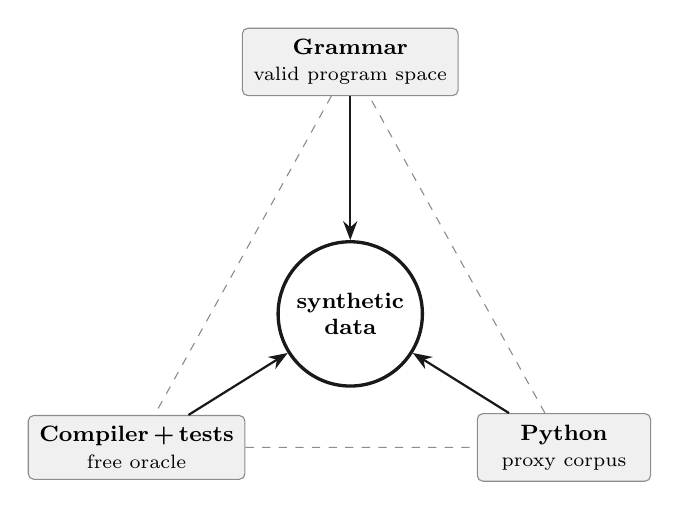
\begin{tikzpicture}[every node/.style={font=\scriptsize}]
        \node[box, minimum width=22mm] (g) at (90:3.2) {\textbf{Grammar}\\\scriptsize valid program space};
        \node[box, minimum width=22mm] (c) at (212:3.2) {\textbf{Compiler\,+\,tests}\\\scriptsize free oracle};
        \node[box, minimum width=22mm] (p) at (328:3.2) {\textbf{Python}\\\scriptsize proxy corpus};
        \node[gate, circle, minimum size=15mm] (s) at (0,0) {synthetic\\data};
        \draw[line, dashed] (g) -- (c) -- (p) -- (g);
        \draw[flow] (g) -- (s); \draw[flow] (c) -- (s); \draw[flow] (p) -- (s);
      \end{tikzpicture}}
      \\[2mm] {\scriptsize the multi PLT method}
    \end{column}
  \end{columns}
  \note{PLT means programming language theory. Three things make 100\% synthetic data
  trustworthy: the grammar bounds what is valid, the compiler and tests label for free at any
  scale, and Python is a huge correct corpus to transpile from. The decision that matters: gate
  on \texttt{jac run}, not \texttt{jac check}. The strict type checker rejects untyped but
  runnable Jac, and that would throw away good data.}
\end{frame}

% ================================================================ 4. DATA TIERS PT1
\begin{frame}{Data tiers, part 1: the three sources}
  \begin{columns}[t]
    \begin{column}{0.6\textwidth}
      \begin{enumerate}
        \item \textbf{Idiomatic core} [147]. Jac written by hand or with an agent (Claude
              Code plus the Jac MCP): walkers, nodes, edges. \emph{31 of these are graph shaped.}
        \item \textbf{Transpile volume} [1500]. Python auto transpiled with \texttt{jac py2jac}
              and gated on behavior. Correct, but \emph{Python shaped}. This is the cheap volume.
        \item \textbf{DPO pairs} [147]. \texttt{chosen} is idiomatic, \texttt{rejected} is the
              transpile. This teaches the model \emph{what is right versus what is wrong}.
      \end{enumerate}
    \end{column}
    \begin{column}{0.4\textwidth}
      \centering
      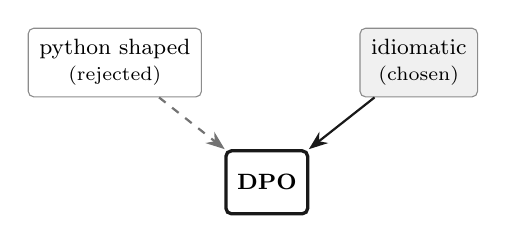
\begin{tikzpicture}[every node/.style={font=\footnotesize}]
        \node[box, fill=white] (p) {python shaped\\\scriptsize (rejected)};
        \node[box, right=20mm of p] (i) {idiomatic\\\scriptsize (chosen)};
        \node[gate, below=11mm of $(p)!0.5!(i)$] (d) {DPO};
        \draw[flow, dashed, color=soft] (p) -- (d);
        \draw[flow] (i) -- (d);
      \end{tikzpicture}
      \\[2mm]{\scriptsize a DPO pair is one task with\\ two answers (chosen $\succ$ rejected)}
    \end{column}
  \end{columns}
  \vspace{2mm}
  \begin{center}\small
   \textbf{1647} SFT examples (147 idiom, 1500 transpile) \,\textbullet\, \textbf{147} DPO pairs
   \,\textbullet\, gate is \texttt{jac run}
  \end{center}
  \note{Two SFT tiers, on purpose. The transpile volume is cheap and large but Python shaped.
  The idiomatic core is small and expensive but Jac shaped. I mix them so the model sees enough
  idiom and does not just learn to transpile. DPO is a third signal, a preference signal layered
  on top. The numbers match the dataset builders, and the 31 graph shaped idiomatic examples are
  what open the idiom axis later.}
\end{frame}

% ================================================================ 5. DATA TIERS PT2
\begin{frame}{Data tiers, part 2: how the tiers are built}
  \begin{center}
  \resizebox{\textwidth}{!}{%
  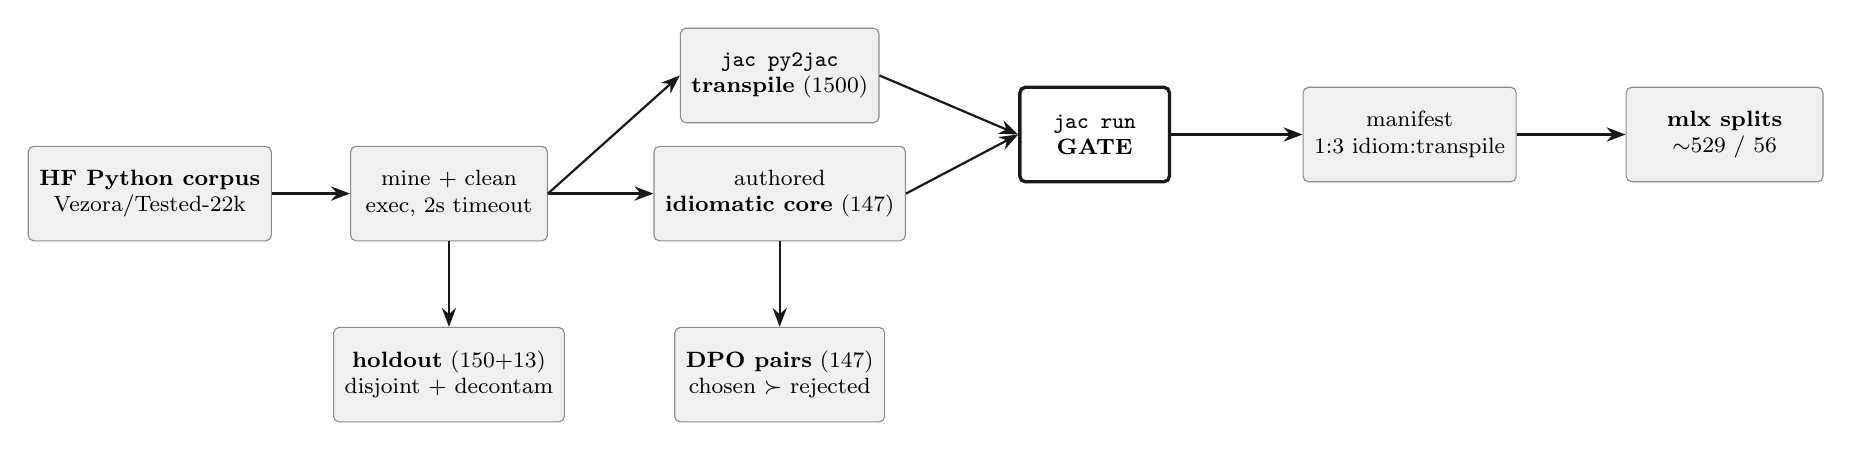
\begin{tikzpicture}[every node/.style={font=\scriptsize, align=center},
                      box/.append style={minimum width=25mm, minimum height=12mm}]
    \node[box] (hf)   at (0,1.3)  {\textbf{HF Python corpus}\\Vezora/Tested-22k};
    \node[box] (mine) at (3.8,1.3){mine + clean\\exec, 2s timeout};
    \node[box] (trans) at (8.0,2.8){\texttt{jac py2jac}\\\textbf{transpile} (1500)};
    \node[box] (core)  at (8.0,1.3){authored\\\textbf{idiomatic core} (147)};
    \node[gate, minimum width=19mm, minimum height=12mm] (gate) at (12.0,2.05){\texttt{jac run}\\GATE};
    \node[box] (man)   at (16.0,2.05){manifest\\1:3 idiom:transpile};
    \node[box] (split) at (20.0,2.05){\textbf{mlx splits}\\$\sim$529 / 56};
    \node[box] (dpo)   at (8.0,-1.0){\textbf{DPO pairs} (147)\\chosen $\succ$ rejected};
    \node[box] (hold)  at (3.8,-1.0){\textbf{holdout} (150+13)\\disjoint + decontam};

    \draw[flow] (hf) -- (mine);
    \draw[flow] (mine.east) -- (trans.west);
    \draw[flow] (mine.east) -- (core.west);
    \draw[flow] (trans.east) -- (gate.west);
    \draw[flow] (core.east)  -- (gate.west);
    \draw[flow] (gate) -- (man);
    \draw[flow] (man) -- (split);
    \draw[flow] (core) -- (dpo);
    \draw[flow] (mine) -- (hold);
  \end{tikzpicture}%
  }
  \end{center}
  \vspace{1mm}
  \begin{center}\small
   \texttt{jac run} gated \,\textbullet\, manifest \textbf{1:3} idiom:transpile \,\textbullet\,
   holdout decontaminated (disjoint offsets, 14 token shingles)
  \end{center}
  \note{This is the build, not just the inventory. Reading across: mine Python, transpile or
  author Jac, gate everything on \texttt{jac run}, balance the manifest at 1:3, split for MLX.
  Two honesty mechanisms worth saying out loud. The 1:3 ratio stops the model collapsing into
  pure transpiling, and the holdout is decontaminated (disjoint corpus offsets plus a 14 token
  shingle overlap check), so the eval numbers are real generalization rather than memorization.
  The DPO pairs are built from the idiomatic core.}
\end{frame}

% ================================================================ 5b. REAL EXAMPLES (SFT)
\begin{frame}[fragile]{The data, tier by tier: real examples (1 of 2)}
  \begin{columns}[t]
    \begin{column}{0.52\textwidth}
      \textbf{Tier 1 \,\textbullet\, Idiomatic core} \;{\scriptsize (authored: walker / node / edge)}\\
      {\scriptsize task: \texttt{product\_of\_tree}, multiply values over a tree}
      \begin{lstlisting}[style=code,language=Jac,basicstyle=\ttfamily\tiny\color{ink}]
node TNode { has val: int; }

walker Product {
    has result: int = 1;
    can mul with TNode entry {
        self.result *= here.val;
        visit [-->];          # the walk IS the program
    }
}

with entry {
    a = TNode(val=2); b = TNode(val=3); c = TNode(val=4);
    root ++> a;  a ++> b;  a ++> c;
    print((a spawn Product()).result);
}
      \end{lstlisting}
    \end{column}
    \begin{column}{0.48\textwidth}
      \textbf{Tier 2 \,\textbullet\, Transpile volume} \;{\scriptsize (\texttt{jac py2jac}, gated)}\\
      {\scriptsize task: \texttt{is\_even}, mechanical, Python shaped}
      \begin{lstlisting}[style=code,language=Jac,basicstyle=\ttfamily\tiny\color{ink}]
def is_even(num: Any) -> object {
    return ((num % 2) == 0);
}

with entry {
    print(is_even(5));
    print(is_even(10));
}
      \end{lstlisting}
      \vspace{1mm}
      {\scriptsize Correct and runnable, but it is just Python with braces: \texttt{Any} and
       \texttt{object} types, no walker. The transpile gives cheap scale. The idiomatic core
       gives the shape.}
    \end{column}
  \end{columns}
  \note{Show it instead of describing it. The left example is real text from sft.jsonl, a graph
  problem whose idiomatic answer builds nodes and spawns a walker, so the traversal is the
  program. The right example is real text from sft\_auto.jsonl, the py2jac output: correct and
  runnable, but Python shaped (Any/object types, a plain def). Both pass the jac run gate. The
  mix is the point: volume from the right, idiom from the left.}
\end{frame}

% ================================================================ 5c. REAL EXAMPLE (DPO)
\begin{frame}[fragile]{The data, tier by tier: a real DPO pair (2 of 2)}
  \begin{center}{\scriptsize task: \texttt{count\_children(graph, node)}, count a node's direct children}\end{center}
  \begin{columns}[t]
    \begin{column}{0.5\textwidth}
      \centering\textbf{chosen} \;{\scriptsize idiomatic $\Rightarrow$ reward $\uparrow$}
      \begin{lstlisting}[style=code,language=Jac,basicstyle=\ttfamily\tiny\color{ink}]
node GNode { has name: str; }

walker CountChildren {
    has count: int = 0;
    can chk with GNode entry {
        self.count = len([-->]);
        disengage;
    }
}
      \end{lstlisting}
    \end{column}
    \begin{column}{0.5\textwidth}
      \centering\textbf{rejected} \;{\scriptsize transpile, Python shaped $\Rightarrow$ reward $\downarrow$}
      \begin{lstlisting}[style=code,language=Jac,basicstyle=\ttfamily\tiny\color{ink}]
"""Return the number of direct
   children of node."""
def count_children(graph: dict,
                   `node: str) -> int {
    return len(graph.get(`node, []));
}
      \end{lstlisting}
    \end{column}
  \end{columns}
  \vspace{1mm}
  \begin{center}\small
   Same task, two correct answers. DPO trains \textbf{chosen $\succ$ rejected}, pushing
   generation off \texttt{graph.get(...)} and toward \texttt{len([-->])}.
  \end{center}
  \note{This is one row of dpo.jsonl. Both versions compile and run; the only difference is
  idiom. The chosen answer reaches across edges with len([-->]) and a walker. The rejected one
  is the transpiled dict.get. DPO needs exactly this: two valid answers that differ on the idiom
  axis. This ties back to the function versus graph slide, because it only has teeth on graph
  shaped tasks, where the two answers genuinely diverge.}
\end{frame}

% ================================================================ 6. SFT vs DPO
\begin{frame}{What is SFT and DPO}
  \begin{columns}[c]
    \begin{column}{0.42\textwidth}
      \begin{itemize}
        \item \textbf{SFT} is supervised finetuning. Imitate gold outputs, which teaches the
              model to \emph{produce runnable Jac}.
        \item \textbf{DPO} is direct preference optimization. Learn from
              \texttt{chosen}\,$\succ$\,\texttt{rejected} pairs, which \emph{sharpens} the model
              toward idiom without a reward model.
      \end{itemize}
      \vspace{2mm}
      {\small Here, SFT teaches it to \emph{run}, and DPO pushes it from \emph{runs} to
       \emph{idiomatic}.}
    \end{column}
    \begin{column}{0.56\textwidth}
      \centering
      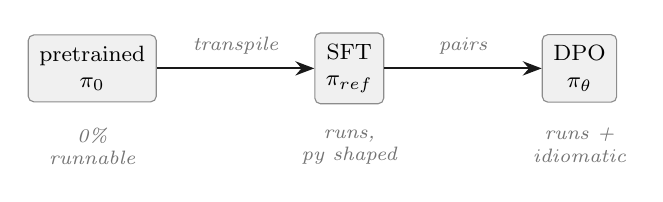
\begin{tikzpicture}[node distance=10mm, every node/.style={font=\footnotesize}]
        \node[box] (base) {pretrained\\$\pi_0$};
        \node[box, right=20mm of base] (sft) {SFT\\$\pi_{\text{ref}}$};
        \node[box, right=20mm of sft] (dpo) {DPO\\$\pi_\theta$};
        \draw[flow] (base) -- node[lbl,above=0.5mm]{transpile} (sft);
        \draw[flow] (sft) -- node[lbl,above=0.5mm]{pairs} (dpo);
        \node[lbl, below=2mm of base, align=center] {0\%\\runnable};
        \node[lbl, below=2mm of sft, align=center] {runs,\\py shaped};
        \node[lbl, below=2mm of dpo, align=center] {runs +\\idiomatic};
      \end{tikzpicture}
    \end{column}
  \end{columns}
  \note{Keep this short. It is just the vocabulary the audience needs for the results. The one
  message: SFT and DPO do different jobs. SFT gets the model to runnable Jac. DPO only moves the
  idiom axis, and only when there is idiom headroom, which is the next slide.}
\end{frame}

% ================================================================ 7. FUNCTION vs GRAPH
\begin{frame}{Function vs graph tasks}
  \begin{columns}[t]
    \begin{column}{0.5\textwidth}
      \centering\textbf{Function task}\\[1mm]
      {\scriptsize standalone pure function $\to$ Jac \texttt{def}}
      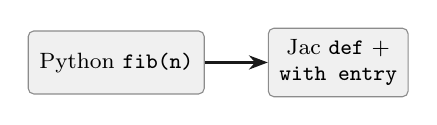
\begin{tikzpicture}[every node/.style={font=\scriptsize}]
        \node[box] (py) {Python \texttt{fib(n)}};
        \node[box, right=8mm of py] (jac) {Jac \texttt{def} +\\\texttt{with entry}};
        \draw[flow] (py) -- (jac);
      \end{tikzpicture}
      \begin{itemize}\scriptsize
        \item idiomatic $\approx$ transpile $\Rightarrow$ \textbf{sim 0.97}
        \item \textbf{no idiom headroom}: a pure function legitimately needs no walker
        \item oracle: recorded test cases (150 holdout)
      \end{itemize}
    \end{column}
    \begin{column}{0.5\textwidth}
      \centering\textbf{Graph task}\\[1mm]
      {\scriptsize dict and stack traversal $\to$ nodes / edges / walker}
      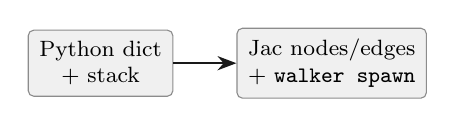
\begin{tikzpicture}[every node/.style={font=\scriptsize}]
        \node[box] (py) {Python dict\\+ stack};
        \node[box, right=8mm of py] (jac) {Jac nodes/edges\\+ \texttt{walker spawn}};
        \draw[flow] (py) -- (jac);
      \end{tikzpicture}
      \begin{itemize}\scriptsize
        \item idiomatic \emph{diverges} hard $\Rightarrow$ \textbf{sim 0.26}, $\sim$8 constructs
        \item \textbf{real idiom headroom}: this is where DPO can move the model
        \item one dict argument keeps the same eval harness (13 holdout)
      \end{itemize}
    \end{column}
  \end{columns}
  \vspace{1mm}
  \begin{center}\small
   The idiom axis only \emph{exists} on graph tasks. On functions, ``Python shaped'' already
   \emph{is} idiomatic, which is why DPO does nothing there and works here.
  \end{center}
  \note{This is the pivot of the whole talk. A pure function like factorial or fib transpiles to
  essentially the idiomatic Jac, similarity 0.97, with nothing for DPO to push toward. A graph
  problem written in Python as a dict and a stack should be rewritten with nodes, edges and a
  walker, and similarity drops to 0.26 with about 8 spatial constructs. I keep one dict argument
  in the signature so the same behavioral harness runs both. The line to land: headroom is a
  property of the task, not the model.}
\end{frame}

% ================================================================ 8. GRAPHS & STATS
\begin{frame}{Graphs and stats: behavioral test pass}
  \begin{columns}[c]
    \begin{column}{0.42\textwidth}
      \begin{itemize}\small
        \item Base eval from \textbf{cold start} (quantized Q4/Q8, run normally).
        \item \textbf{Base is 0\%}: neither model knew Jac before this.
        \item Functions: both reach \textbf{$\sim$94\%}. SFT and DPO tie, outputs stay Python
              shaped, and DPO does not move them.
        \item Graph: \textbf{Qwen pulls ahead} (46/61\%) while Gemma stalls (15\%).
      \end{itemize}
    \end{column}
    \begin{column}{0.58\textwidth}
      \centering
      
\includegraphics[width=\linewidth]{figs/accuracy_compare.png}
    \end{column}
  \end{columns}
  \note{The headline chart. Read the bars left to right: function base 0/0, function SFT 94/93,
  function DPO 93/93 (flat, no headroom), graph SFT 46 vs 15, graph DPO 61 vs 15. Two stories in
  one figure. Functions are a tie and DPO is flat there. Graph is where the models separate and
  where DPO pays off, but only for Qwen.}
\end{frame}

% ================================================================ 9. GRAPHS & STATS PT2
\begin{frame}{Graphs and stats, part 2: training curves}
  \begin{columns}[c]
    \begin{column}{0.32\textwidth}
      \small Validation loss, training loss, and the holdout learning curve are
      \textbf{nearly identical} for Qwen and Gemma. Same data, same config
      (LoRA r16, 600 iters, lr 2e-5).
      \\[2mm]
      {\footnotesize The separation is \emph{not} in loss. It is in \emph{idiom} on graph tasks,
       which is the next slide.}
    \end{column}
    \begin{column}{0.68\textwidth}
      \centering
      
\includegraphics[width=0.49\linewidth]{figs/learning_curve_compare.png}\hfill
      
\includegraphics[width=0.49\linewidth]{figs/train_loss_compare.png}\\[1mm]
      
\includegraphics[width=0.49\linewidth]{figs/val_loss_compare.png}
    \end{column}
  \end{columns}
  \note{These curves answer the question "did one model just train better?" No. Train loss, val
  loss and the per checkpoint holdout learning curve overlap almost exactly, so the optimization
  is the same. That means the graph idiom gap on the next slide is a real capability difference,
  not a training artifact.}
\end{frame}

% ================================================================ 10. GRAPH TIER IDIOM
\begin{frame}{Graph tier: where idiom has room to move}
  \begin{columns}[c]
    \begin{column}{0.5\textwidth}
      \begin{itemize}\small
        \item On graph tasks idiomatic Jac \emph{diverges} from Python, so the idiom axis is
              alive.
        \item \textbf{SFT} teaches the model to \emph{run}. \textbf{DPO} pushes it the rest of
              the way to \emph{idiomatic}.
        \item \textbf{Qwen}: SFT 46\% $\rightarrow$ DPO \textbf{61\%} correct; idiomatic share of
              correct 83\% $\rightarrow$ \textbf{100\%}; similarity 0.457 $\rightarrow$
              \textbf{0.338} (ref 0.26).
        \item \textbf{Gemma}: graph SFT only 15\% ($\sim$2/13, 0 constructs), so DPO has nothing
              to move. Idiom acquisition depends on the model.
      \end{itemize}
    \end{column}
    \begin{column}{0.5\textwidth}
      \centering
      
\includegraphics[width=\linewidth]{figs/graph_idiom_compare.png}
    \end{column}
  \end{columns}
  \note{The payoff slide. Bars are graph correctness, lines are transpile similarity, where lower
  means more idiomatic. For Qwen, DPO lifts correctness from 46 to 61 and drives 100\% of correct
  outputs to idiomatic, with similarity sliding toward the 0.26 reference. Gemma's graph SFT is
  too weak for DPO to bite, which confirms the rule: DPO sharpens idiom that SFT already produced,
  it cannot manufacture it. Practical takeaway: pick Qwen3 Coder for Jac graph idiom.}
\end{frame}

% ================================================================ 11. WHAT WE PROVED
\begin{frame}{What we proved}
  \begin{enumerate}
    \item \textbf{Synthetic, compiler validated data teaches correct Jac.} 0\%
          $\rightarrow$ \textbf{94\%} behavioral test pass on a decontaminated holdout.
    \item \textbf{Idiom headroom plus DPO teaches idiomatic Jac.} On graph tasks Qwen3 Coder
          reaches \textbf{100\%} idiomatic of correct outputs, up from 83\% at SFT.
    \item \textbf{The result is a basic Jac coding agent.} Roughly what Claude Code is, but for
          Jac instead of Python.
  \end{enumerate}
  \vspace{3mm}
  \begin{center}\small\color{soft}
    100\% synthetic data \,\textbullet\, a free compiler oracle \,\textbullet\, two MoE models that fit in 48\,GB
  \end{center}
  \note{The summary in three lines. Line 1 is the SFT result on behavior. Line 2 is the DPO and
  idiom result on the tier that has headroom. Line 3 is the point: this pipeline produces a usable
  Jac code model starting from zero corpus.}
\end{frame}

% ================================================================ 12. NEXT UP
\begin{frame}{Next up}
  \begin{columns}[T]
    \begin{column}{0.62\textwidth}
      \begin{itemize}\small
        \item Mine a single codebase into an \textbf{RL loop}: how far is the resulting codebase
              from what you asked for?
        \item Is it unreasonable to train a model on \emph{one} codebase?
        \item What \textbf{eval} fits that setting?
      \end{itemize}
    \end{column}
    \begin{column}{0.38\textwidth}
      {\footnotesize\textbf{Shipped since:} a live \textbf{training dashboard} (Monitor, Train,
       Ingest) that streams SFT and DPO runs in real time. It is the item that was ``next'' last
       time.}
    \end{column}
  \end{columns}
  \vspace{1mm}
  \begin{center}
    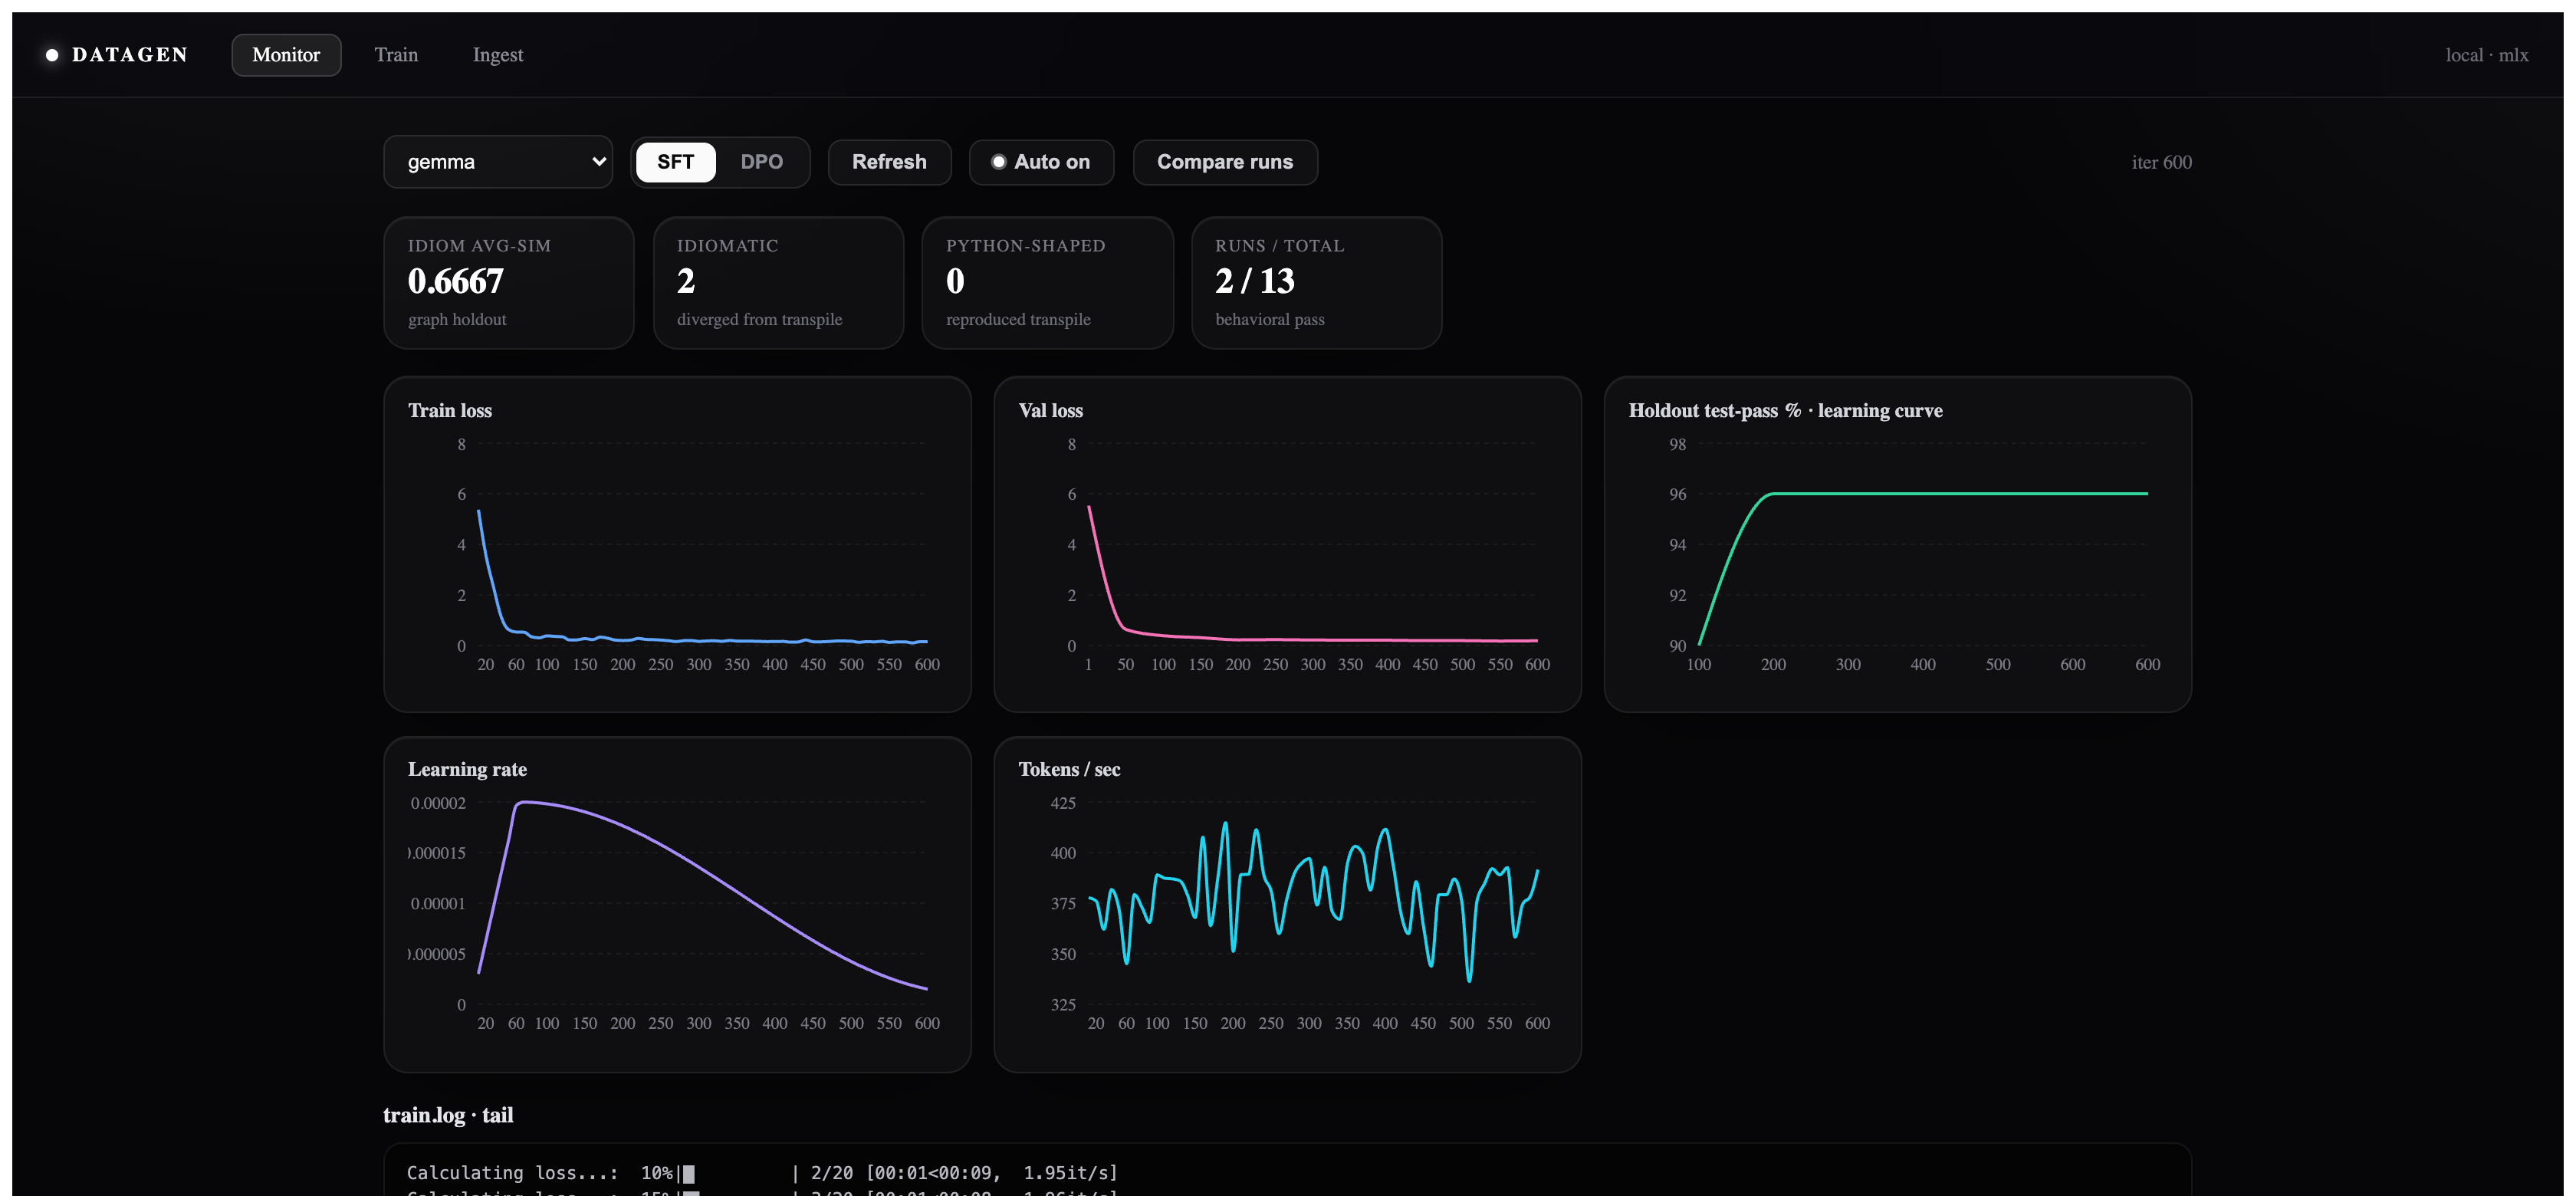
\includegraphics[width=0.88\textwidth]{figs/dashboard_wide.png}
    \\[0.5mm]{\scriptsize live Monitor: run picker, idiom cards, train and val loss, learning curve, tok/s}
  \end{center}
  \note{Close on direction, not a recap. The open research question is the single codebase RL
  loop and what eval even means there. Then the concrete part: the dashboard I promised last time
  is built. The banner is the live Monitor screen from the jac client app, with gemma selected,
  the idiom cards, and five charts. If you do not want the screenshot, drop it and the RL loop
  questions stand on their own.}
\end{frame}

\end{document}
